\chapter{Datasets}
Procediamo ora a descrivere i dataset contenenti dati di telemetrie registrati negli anni e resi pubblici in modo da poter sperimentare e migliorare gli algoritmi già presenti.

\section{Dataset ESA}

Il dataset di riferimento più importante per la rilevazione delle anomalie è quello fornito dall'ESA (European Space Agency) che conta dati di tre missioni. Di queste solo i dati di due vengono utilizzati per creare il benchmark, per le caratteristiche dell'insieme di dati; infatti in \textit{"Mission 3"} abbiamo: poche anomalie e per lo più banali, un gran numero di buchi di comunicazione e segmenti non validi.

Nell'articolo$^{\text{\cite{ESA_benchmark}}}$ in questione i dati satellitari grezzi di \textit{"Mission 1"} e \textit{"Mission 2"} vengono preprocessati per renderli uniformi e quindi utilizzabili con la maggior parte degli algoritmi.

In questa fase è stato utilizzato lo strumento OXI$^{\text{\cite{OXI_annotation_tool}}}$ per l'etichettatura collaborativa dei dati da cui si è potuto estrarre delle telemetrie che rappresentano periodi di funzionamento nominale e anomalo. Tutti i dati sono stati sottoposti ad una doppia fase di etichettatura e controllo.

I canali sono divisi tra "target" e "non target", dove quest'ultimi sono usati per gli algoritmi solo come informazioni addizionali. Un canale target, quello usato per rilevare le anomalie, è diviso in gruppi di dati con caratteristiche simili così da rendere più facile per l'algoritmo processarli ed interpretarli e, nel caso, allenarlo solo su quel gruppo specifico.
\pagebreak

\begin{table}[h!]
    \centering
    \begin{tabular}{|l|c|c|}
        \hline
         \textbf{}& \textbf{Mission 1} & \textbf{Mission 2}\\
         \hline
        \textbf{Channels} & 76 & 100\\
        Target/Non target & 58/18 & 47/53\\
        \hline
        \textbf{Telecommands} & 698 & 123\\
        \hline
        \textbf{Annotate Events} & 200 & 644 \\
        Anomalies& 118 & 31\\
        Rare Nominal Events &78  & 613\\
        Univariate/Multivariate& 32/164 & 9/635\\
        \hline
    \end{tabular}
    \caption{Configurazione Dataset ESA}
    \label{tab:costituzioneESA_dataset}
\end{table}

Possiamo osservare dalla Tabella \ref{tab:costituzioneESA_dataset} che la densità di anomalie in termini di punti di dati annotati, varia tra $0,57\%$ per la \textit{"Mission 2"} e $1,80\%$ per la \textit{"Mission 1"} questo va a confermare un'impronta più realistica rispetto ai dataset meno recenti che avevano una densità di anomalie estremamente più alta ed irrealistica.

\section{Dataset NASA}
Il dataset NASA riporta i dati provenienti da missioni reali effettuate negli anni, questi coprono più aspetti relativi al contesto spaziale con il conseguente aumento di complessità.

Il dataset contiene serie temporali con numerosi parametri di telemetria, tra cui eventi normali e anomali.
Le anomalie sono rare, infatti possiamo riscontrare canali che non ne possiedono nemmeno una, rappresentando una sfida significativa, insieme anche al fatto che non tutti i dati sono etichettati.

Elenchiamo alcune particolarità e soprattutto sfide:
\begin{itemize}
    \item Rarità: le anomalie presenti nel dataset sono in quantità ridotta, rendendo l'addestramento dei modelli più difficile;
    \item Etichettatura: le etichettature dei dati sono incomplete, complicando ulteriormente l'identificazione;
    \item Rumorosità: i dati presenti, a causa anche della provenienza da diverse missioni, contengono lacune e sono spesso rumorosi a causa di fattori esterni;
    \item Variabilità: i parametri variano molto;
    \item Veridicità: i dati rispecchiano la realtà, portando così a poter testare i modelli in un contesto simile ai dati reali.
\end{itemize}

Utilizziamo questo dataset perché permette di utilizzare dati realistici, valutando in maniera più accurata gli algoritmi proposti. Inoltre, utilizzare un dataset con molteplici sperimentazioni e test effettuati, permette di avere un confronto diretto dei modelli, potendo anche validare i risultati ottenuti, aumentando la credibilità e avvalorando le analisi proposte da altri o la possibilità che altri validino le nostre.

\section{Motivazioni}
Il dataset ESA precedentemente descritto porta alla risoluzione di vari problemi noti nell'ambito della rilevazione di anomalie.
Il primo problema, relativo al dataset NASA, è la loro struttura, come si evidenzia nei dataset \textit{NASA Soil Moisture Active Passive} (SMAP) e  \textit{Mars Science Laboratory} (MSL), i quali offrono brevi frammenti di segnali e comandi correlati da, rispettivamente, 55 e 27 parametri di telemetria, con un totale di 105 anomalie annotate; infatti abbiamo una densità di anomalie irrealistica, alto numero di anomalie banali, verità di base etichettate in maniera errate ed una mancanza di correlazione tra comandi e canali. 
% Come conseguenza di questo è stato deciso che questi dataset non andrebbero usati per il benchmarking del rilevamento delle anomalie.
Il secondo problema invece rappresenta la mancanza di annotazione di eventi anomali, alcuni esempi sono gli insiemi di dati di \textit{Mars Express6} e \textit{NASA WebTCAD7}.

Il dataset ESA risolve i problemi elencati, ma nasce come dataset di missioni su larga scala, le quali sono molto complesse e stabili, portando con sé problemi non più relativi alla distribuzione delle anomalie, ma improntati verso difficoltà di esecuzione e potenza di calcolo.

Il dataset che introdurremo successivamente è concettualmente diverso, infatti affronta una missione ESA OPS\textunderscore SAT molto semplificata, al fine di renderne più accessibile l'uso, oltre ad essere di dimensione considerevolmente minore.

Questo processo di apertura è reso anche tramite la sostituzione giornaliera dell'intero sistema software fino al sistema operativo del satellite, così da consentire ai ricercatori di caricare il proprio software a bordo del satellite. Per implementare questa funzionalità venne usato FDIR$^{\text{\cite{FDIR}}}$ (Fault Detection, Isolation, and Recovery), un metodo che rileva, isola e corregge automaticamente i malfunzionamenti, assicurando il funzionamento continuo del satellite e permettendo una gestione dinamica delle sue funzionalità.

Le telemetrie grezze sono caratterizzate da molte lacune nei dati ed altre imprecisioni, queste vengono curate da ingegneri ed esperti nei modelli di apprendimento automatico per rendere l'insieme di dati fruibile alla creazione di tecniche di rilevamento delle anomalie basate su di essi.
Una di queste modifiche è la seguente:

\begin{quote}
    Selezione e annotazione di verità di base (ground\textunderscore truth) di 2123 brevi frammenti di telemetria a canale singolo, ossia serie temporali univariate$^{\text{\cite{OPS-SAT}}}$, registrate in 9 canali di telemetria.
\end{quote}

Infine questo dataset, con il relativo benchmark e tutti i dati disponibili al suo interno, è stato messo a disposizione per aiutare la comunità nella ricerca di nuovi approcci per la rilevazione delle anomalie, confrontandosi tra di loro in modo imparziale ed equo, così da affrontare anche il problema della riproducibilità nell'ambiente dell'apprendimento automatico (dato che i dataset sono uniformati, l'ambiente di esecuzione potrebbe essere diverso e sono state utilizzate varie metriche). 

Tutto ciò che è stato sviluppato con l'aiuto del dataset verrà convalidato con il lancio alla fine del 2025 del satellite successore OPS\textunderscore SAT VOLT (dopo aver distribuito i vari modelli a bordo del satellite).


\section{OPS-SAT Dataset}
Nel dataset OPS\textunderscore SAT sono contenuti i dati delle telemetrie del satellite OPS\textunderscore SAT dell'ESA (Figura \ref{fig:OP-SAT_satellite}). Questo satellite di tipo CubeSat aveva dimensione 3 unità (3U dove 1U=10cm$^3$); esso ormai non è più in orbita, era stato lanciato a Dicembre del 2019 con lo scopo di dimostrare l'elaborazione dei dati in orbita e di generare dati utili come immagini satellitari e telemetrie.

\begin{figure}[ht]
    \centering
    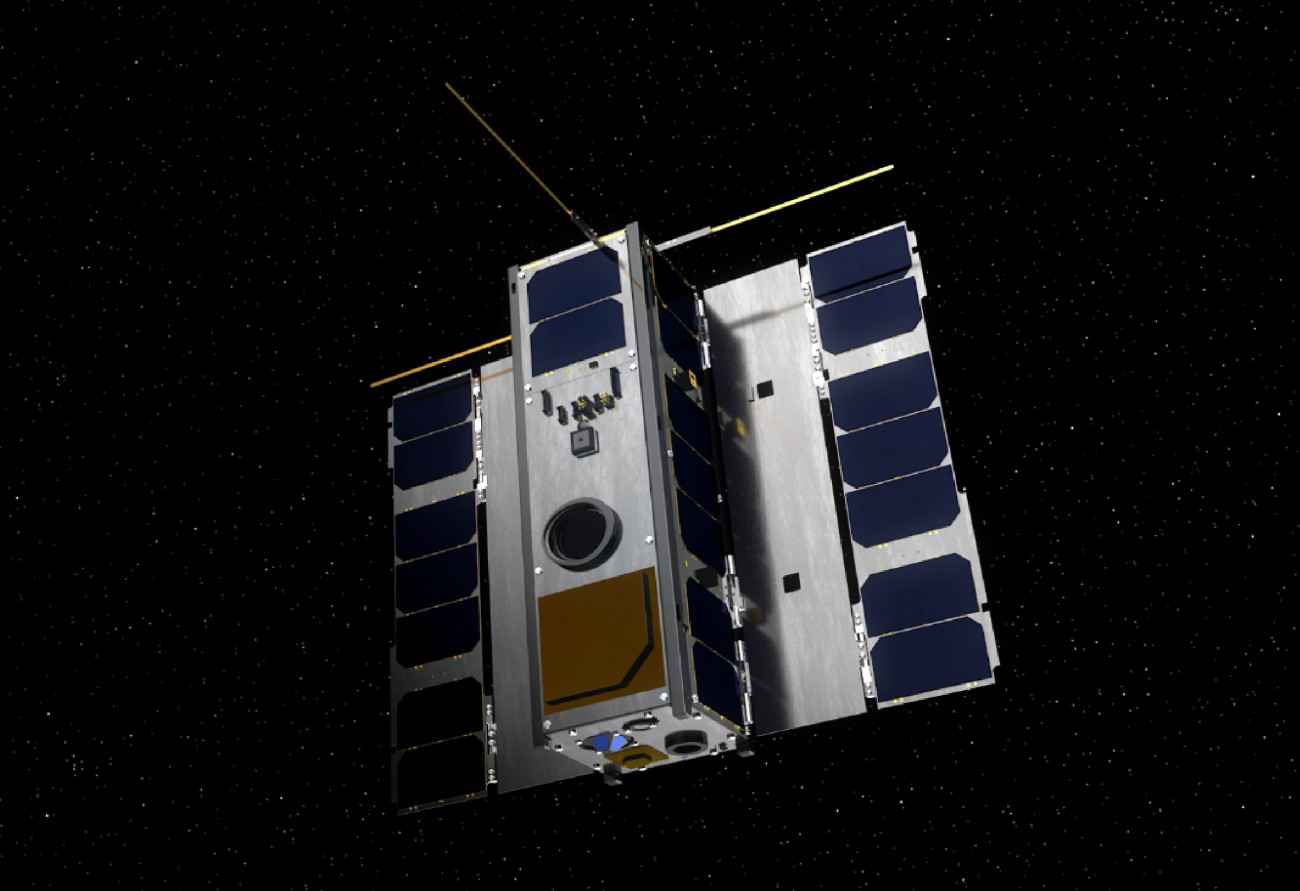
\includegraphics[width=0.5\linewidth]{images/Capitolo2/OP-SAT_satellite.png}
    \caption{Satellite OPS\textunderscore SAT. Fonte: European Space Agency}
    \label{fig:OP-SAT_satellite}
\end{figure}

Come nel dataset precedente anche qui i dati hanno bisogno di essere preprocessati per renderli fruibili alla maggior parte degli algoritmi (OXI$^{\text{\cite{OXI_annotation_tool}}}$). In questo caso sono state progettate 18 caratteristiche per l'attività di rilevamento delle anomalie, ossia sono stati estratti tratti significativi dai dati. Questo processo è chiamato Feature Extraction e serve per ridurre la complessità dei dati in ingresso, rendendoli più significativi.

Tutti i segmenti ricavati rappresentano le sfide che dobbiamo affrontare con i dati delle telemetrie, ognuno di questi è composto da:
\begin{itemize}
    \item $\langle$\texttt{timestamp}$\rangle$: rappresenta il marcatore temporale nel momento della registrazione;
    \item $\langle$\texttt{channel}$\rangle$: è il nome del canale;
    \item $\langle$\texttt{value}$\rangle$: è il valore del segnale acquisito;
    \item $\langle$\texttt{label}$\rangle$: rappresentano le annotazioni certe, quelle annotate manualmente;
    \item $\langle$\texttt{segment}$\rangle$: rappresenta il numero consecutivo del segmento;
    \item $\langle$\texttt{sampling}$\rangle$: è il tasso di campionamento;
    \item $\langle$\texttt{train}$\rangle$: indica se il segmento appartiene al training set.
    
\end{itemize}

Il dataset è stato diviso in una parte di allenamento, Training Set ($T$), ed una di test, Test Set ($\Psi$). Questi rappresentano rispettivamente i dati usati per l'allenamento del modello e i dati usati per fare le valutazioni delle performance dell'algoritmo.

\begin{table}[h!]
    \centering
    \begin{tabular}{|l|c|c|c|}
        \hline
        \textbf{Classi} &\textbf{Training Set} ($T$) & \textbf{Test Set ($\Psi$)}&\textbf{Total} \\
        \hline
         Nominali& 1273&416 &1689 \\
         Anomalie& 321&529 &434\\
         \hline
    \end{tabular}
    \caption{Composizione Dataset OPS\textunderscore SAT}
    \label{tab:dataset_op-sat}
\end{table}

Le classi mostrate in Tabella \ref{tab:dataset_op-sat}, nominali e anomalie, rappresentano rispettivamente segmenti che rispettano valori normali o attesi e segmenti invece che superano questi valori o discordano dai valori attesi.

Partendo dai benchmark effettuati su NASA ed OPS\textunderscore SAT, analizzeremo le metriche e le prestazioni utilizzando vari modelli per il rilevamento delle anomalie, partendo dal secondo dataset (OPS\textunderscore SAT), che contiene dati più semplici per il nostro obiettivo, per poi dedicarci a NASA per finire.

\section{Validazione Paper OPS\textunderscore SAT}
In questa sezione vogliamo verificare le prestazioni di tutti gli algoritmi presenti nel paper relativo ad OPS\textunderscore SAT, questo per avere un confronto con le metriche risultanti degli algoritmi che vedremo successivamente.

I dati che utilizziamo sono estratti tramite le funzioni rese disponibili dal paper, partendo quindi già con i dati elaborati e divisi in \texttt{X\textunderscore train, X\textunderscore test, y\textunderscore train, y\textunderscore test}.
Tramite la funzione \texttt{StandardScaler()} scaliamo i dati, ottenendo le metriche desiderate, riportate nella tabella sottostante.
\vspace{0.5cm}
\begin{table}[h]
    \centering
    \begin{adjustbox}{max width=\textwidth}
        \begin{tabular}{|c|c|c|c|c|c|c|c|c|}
        \hline
            \textbf{Modello} & \textbf{Accuracy} &\textbf{Precision}  & \textbf{Recall} & \textbf{F1} & \textbf{MCC} & \textbf{AUC-PR} & \textbf{AUC-ROC} & \textbf{N-Score}\\
            \hline
            \multicolumn{9}{|c|}{\textbf{Supervised}} \\
            \hline
            \textbf{LinearSVC} & 0.926 & 0.911 & 0.726 &0.808  & 0.771 & 0.949 & 0.976 &0.867 \\
            \hline
             \textbf{LogisticRegression}& 0.924 & 0.92 & 0.708 & 0.8 & 0.764 & 0.949 & 0.976 & 0.867 \\
             \hline
             \textbf{FCNN}& 0.96 & 0.926 & 0.885 & 0.905 & 0.88 & 0.963 & 0.982 & 0.903 \\
             \hline
             \textbf{AdaBoost}& 0.934 & 0.89 & 0.788 & 0.836 & 0.797 & 0.923 & 0.962 & 0.841 \\
             \hline
             \textbf{RF+ICCS}& 0.964 &\textbf{ 0.98} & 0.85 & 0.91 & 0.891 & 0.949 & 0.976 & 0.867 \\
             \hline
             \textbf{Linear+L2}& 0.902 & 0.969 & 0.558 & 0.708 & 0.69 & 0.889 & 0.95 & 0.814 \\
             \hline
             \textbf{XGBOD}& \textbf{0.968} & 0.953 & \textbf{0.894} & \textbf{0.922} & \textbf{0.903} & \textbf{0.969} & \textbf{0.99} & \textbf{0.912} \\
             \hline
             \multicolumn{9}{|c|}{\textbf{Unsupervised}} \\
             \hline
             \textbf{MO-GAAL} & \textbf{0.896 }& 0.939 & 0.549 &\textbf{0.693}  & \textbf{0.669} & \textbf{0.771} & 0.849 &0.699 \\
        \hline
         \textbf{AnoGAN}& 0.594 & 0.296 & \textbf{0.655} & 0.408 & 0.19 & 0.403 & 0.651 & 0.239 \\
         \hline
         \textbf{SO-GAAL}& 0.89 & 0.937 & 0.522 & 0.67 & 0.649 & 0.858 & \textbf{0.919} & \textbf{0.761} \\
         \hline
         \textbf{IForest}& 0.701 & 0.297 & 0.292 & 0.295 & 0.105 & 0.347 & 0.635 & 0.301 \\
         \hline
         \textbf{KNN}& 0.849 & 0.78 & 0.407 & 0.535 & 0.489 & 0.658 & 0.852 & 0.593 \\
         \hline
         \textbf{OCSVM}& 0.837 & 0.721 & 0.389 & 0.506 & 0.447 & 0.659 & 0.788 & 0.655 \\
         \hline
         \textbf{ABOD}& 0.845 & 0.782 & 0.381 & 0.512 & 0.472 & 0.644 & 0.843 & 0.584 \\
         \hline
         \textbf{INNE}& 0.83 & 0.689 & 0.372 & 0.483 & 0.418 & 0.624 & 0.801 & 0.646 \\
         \hline
         \textbf{ALAD}& 0.819 & 0.667 & 0.301 & 0.415 & 0.361 & 0.537 & 0.7 & 0.451 \\
         \hline
         \textbf{LMDD}& 0.822 & \textbf{1.0} & 0.168 & 0.288 & 0.37 & 0.624 & 0.765 & 0.663 \\
         \hline
         \textbf{SOD}& 0.826 & 0.611 & 0.513 & 0.558 & 0.453 & 0.621 & 0.797 & 0.549 \\
         \hline
         \textbf{COF}& 0.834 & 0.667 & 0.442 & 0.532 & 0.449 & 0.603 & 0.774 & 0.593 \\
         \hline
         \textbf{LODA}& 0.83 & 0.689 & 0.372 & 0.483 & 0.418 & 0.549 & 0.692 & 0.522 \\
         \hline
         \textbf{LUNAR}& 0.819 & 0.743 & 0.23 & 0.351 & 0.313 & 0.541 & 0.797 & 0.46 \\
         \hline
         \textbf{CBLOF}& 0.802 & 0.569 & 0.292 & 0.386 & 0.304 & 0.45 & 0.574 & 0.372 \\
         \hline
         \textbf{DIF}& 0.788 & \textbf{1.0} & 0.009 & 0.018 & 0.084 & 0.494 & 0.805 & 0.522 \\
         \hline
         \textbf{VAE}& 0.794 & 0.532 & 0.292 & 0.377 & 0.283 & 0.446 & 0.687 & 0.513 \\
         \hline
         \textbf{GMM}& 0.783 & 0.482 & 0.239 & 0.32 & 0.225 & 0.426 & 0.713 & 0.389 \\
         \hline
         \textbf{DeepSVDD}& 0.788 & 0.509 & 0.239 & 0.325 & 0.241 & 0.344 & 0.55 & 0.336 \\
         \hline
         \textbf{PCA}& 0.779 & 0.464 & 0.23 & 0.308 & 0.21 & 0.373 & 0.612 & 0.363 \\
         \hline
         \textbf{COPOD}& 0.767 & 0.4 & 0.177 & 0.245 & 0.147 & 0.328 & 0.627 & 0.257 \\
         \hline
         \textbf{SOS}& 0.758 & 0.364 & 0.177 & 0.238 & 0.125 & 0.308 & 0.524 & 0.274 \\
         \hline
         \textbf{ECOD}& 0.767 & 0.396 & 0.168 & 0.236 & 0.14 & 0.34 & 0.637 & 0.345 \\
         \hline
        \end{tabular}
    \end{adjustbox}
    \caption{Risultati esecuzione di tutti gli algoritmi del benchmark OPS\textunderscore SAT}
    \label{tab:tabella_inizialeOPS_SAT}   
\end{table}
\section{XGBOD}
% Scrivere introduzione all'analisi di XGBOD come stato dell'arte
Partendo dai risultati ottenuti per la validazione del paper OPS\textunderscore SAT, prendiamo in analisi il modello XGBOD, per poter effettuare un confronto con le metodologie che proporremo successivamente effettuando test e analizzando i risultati ottenuti.

XGBOD (eXtreme Gradient Boosting for Outlier Detection) è un algoritmo composto da tre fasi:
\begin{enumerate}
    \item Generazione di nuove rappresentazioni di dati: vengono applicati vari metodi di rilevamento di anomalie non supervisionati ai dati originali, per ottenere punteggi di anomalie, questi rappresentano la nuova vista dei dati;
    \item Selezione dei punteggi rilevanti: i punteggi ottenuti nella fase precedente vengono filtrati per usare solo quelli utili, quest'ultimi sono combinati con le caratteristiche iniziali, creando un nuovo spazio delle caratteristiche arricchito;
    \item Addestramento del modello XGBoost: viene addestrato il modello XGBoost su questo nuovo spazio delle caratteristiche e le previsioni che otteniamo determinano se ogni dato è un'anomalia o no.
\end{enumerate}
Utilizziamo XGBOD invece che XGBoost direttamente perché quest'ultimo, essendo un modello supervisionato, ha bisogno di dati etichettati e soprattutto con anomalie rare, non facili da etichettare.

XGBOD aggiunge una parte di preprocessing, aumenta le informazioni del set di dati con punteggi di anomalie ed utilizza metodi di rilevamento non supervisionato come Isolation Forest, Local Outlier Factor, ecc..

\subsection{XGBoost}
Il modello XGBoost di tipo supervisionato, si sviluppa con un processo iterativo di addestramento di alberi decisionali deboli (alberi decisionali poco profondi e quindi poco accurati), questi vengono combinati tra di loro portando un miglioramento progressivo delle prestazioni del modello.

XGBoost è composto da pochi passi ma ripetuti iterativamente: come primo passo vengono calcolati i residui, la differenza tra le previsioni iniziali ed i valori reali; questi sono i valori che vogliamo ridurre. Con questi valori il modello addestra un insieme di alberi decisionali deboli, dove ognuno cerca di correggere questi valori migliorando le previsioni del modello precedente. Tutti gli alberi vengono aggiunti al modello complessivo di XGBoost, che aggiorna le sue previsioni combinando tutti gli alberi precedentemente costruiti.

Per regolare tutto questo processo, sono applicate internamente tecniche di limitazione e regolazione per evitare un overfitting del modello. All'interno di XGBoost è presente anche una metrica chiamata \textit{tasso di apprendimento}, che permette di decidere quanto un albero incide sul risultato finale, minimizzando così gli errori di percorso.

\subsection{Risultati ottenuti}
Qui sono elencati i risultati ottenuti effettuando varie prove con parametri diversi per ottimizzare XGBOD ed ottenere il miglior compromesso tra efficienza ed efficacia.
\vspace{0.4cm}
\begin{table}[h!]
    \centering
    \begin{adjustbox}{max width=\textwidth}
        \begin{tabular}{|c|c|c|c|c|c|c|c|c|c|}
        \hline
        \textbf{Modello} & \textbf{Accuracy} &\textbf{Precision}  & \textbf{Recall} & \textbf{F1} & \textbf{MCC} & \textbf{AUC-PR} & \textbf{AUC-ROC} & \textbf{Nscore} & \textbf{Tempo}\\
     \hline
            \textbf{M+P} & \textbf{0.97} & 0.945 & \textbf{0.912} &\textbf{0.928}  & \textbf{0.909} & 0.973 & 0.992 &0.92 & \textbf{1.5s}\\
            \hline
             \textbf{Early}& \textbf{0.97} & 0.971 & 0.885 & 0.926 & \textbf{0.909} & 0.969 & 0.99 & 0.912 & 11.3s\\
             \hline
             \textbf{+M}& 0.968 & 0.944 & 0.903 & 0.923 & 0.903 & 0.974 & 0.91 & 0.92 & 3.3s\\
             \hline
             \textbf{P}& 0.964 & 0.943 & 0.885 & 0.913 & 0.891 & 0.972 & \textbf{0.991} & 0.912 &9.8s\\
             \hline
             \textbf{Senza P}& 0.962 & 0.935 & 0.885 & 0.909 & 0.886 & \textbf{0.977} & 0.992 & 0.912 &9.7s\\
             \hline
             \textbf{Grid}& 0.947 & \textbf{0.989} & 0.761 & 0.86 & 0.839 & 0.898 & 0.945 & \textbf{0.969} &45.9s \\
             \hline
        \end{tabular}
    \end{adjustbox}
    \caption{Prove esecuzione di XGBOD}
    \label{tab:XGBOD_table}
\end{table}
\pagebreak

LEGENDA:
\begin{itemize}
    \item M+P: indica l'utilizzo di più modelli, oltre a quelli utilizzati di default,   combinati all'uso di parametri, questo per migliorare le prestazioni complessive;
    \item Grid: è una tecnica che esplora tutte le possibili combinazioni di iperparametri predefiniti (n\textunderscore estimators, max\textunderscore depth e learning\textunderscore rate) per trovare la configurazione che restituisce i migliori risultati;
    \item EarlyStop: viene utilizzato un meccanismo di EarlyStop che ferma l'esecuzione dell'algoritmo quando gli iperparametri non migliorano più per un numero definito di cicli.
\end{itemize}

Dalla Tabella \ref{tab:XGBOD_table} possiamo vedere che il miglior risultato è quello che utilizza più modelli per l'addestramento ed i parametri modificati al fine di efficientare l'esecuzione. Oltre ad avere degli ottimi risultati, l'esecuzione rimane praticamente istantanea sul nostro dataset di esempio OPS\textunderscore SAT.